\begin{problem}
  {Q1(a)}
  \textbf{Prove or disprove} \\
  Claim: Consider an implementation of Ford-Fulkerson algorithm which does not create any backward edges in the residual graph. It is claimed that, there exists a constant $\alpha > 0$, such
  that for any flow network $G$, this modified implementation is guaranteed to find a flow of value at least $\alpha$ times the maximum-flow value in $G$
  \textbf{False} \\
  \begin{proof}
  A method of constructing a graph in which a particular execution of the above algorithm can produce a "max" flow of $1$ whereas the max flow of the graph is an arbitrary positive integer. \\
  First, begin with a graph consisting of 3 nodes, $s,a,t$, as shown in \textbf{Figure A} \\
  The only possible flow of this graph generated by the above algorithm is trivially $f = 1 = \frac{1}{1}$ \\
  Next, add an additional edge $b$, with three additional edges: $(s, b)$ with capacity 1, $(b, a)$ with capacity $1$, and $(b, t)$ with capacity $1$. This is shown in \textbf{Figure B} \\
  The max flow of this graph is $f = 2$. Suppose the above algorithm begins by choosing path $(s, b, a, t)$. The residual graph would contain only edges $(s, a), (b, t)$, so there exists no path from $s-t$ \\
  Therefore, the flow returned by the above algorithm is $f = 1 < 2$ \\
  Now, for $i = 2...\infty$ do:
  Add 3 additional nodes $x, y, z$. Let the current sink be denoted as $w$. \\
  Node $x$ will be the new sink $t$. An edge, $(w, x)$ will be added with capacity i (the previous max flow). \\
  Node $y$ will have edges $(w, y)$ with capacity 2, and $(y, z)$ with capacity 1. \\
  Node $z$ will have edges $(s, z)$ with capacity 1, and $(z, y)$ with capacity 1. \\
  This new graph has a max flow of $i+1$. Simply take the previous max flow, send $i$ flow over the edge $(w, x)$, and 1 flow along the path $(s, z, y, t)$ \\
  However, suppose the algorithm found a "max" flow of value $1$ in the previous iteration (which is trivially possible by induction on $i$). \\
  Take the path used by this "max" flow and add the edges $(w, y)$ with flow $1$, and $(y, x)$ with flow $1$ to the path. \\
  This new path, when explored first by the algorithm, causes the residual graph to have no path from $s$ to $t$, as there exists no path from $z$ to $x$ since $(y, x)$ is removed,
  and by induction the original graph similarly contains no path from any node $n \neq b$ to $w$, and adding $x, y, z$ does not create any new paths from nodes in the original graph to $w$. \\
  2 additional iterations of this construction are shown below in figures \textbf{C, D} \\
  The blue edges with bolded edge weights indicate the first path explored by the algorithm. \\
  If not otherwise specified, the flow across any arbitrary bolded edge is the same as the capacity of the edge. \\
  This was done because drawing pictures in~~\LaTeX~~is hard. \\
  \vspace{5mm}
  \textbf{Figure A}
  \begin{center}
  \begin{tikzpicture}[scale=0.2]
  \tikzstyle{every node}+=[inner sep=0pt]
  \draw [black] (5.1,-51.7) circle (3);
  \draw (5.1,-51.7) node {$s$};
  \draw [black] (22.2,-51.7) circle (3);
  \draw (22.2,-51.7) node {$a$};
  \draw [black] (35.3,-40.4) circle (3);
  \draw (35.3,-40.4) node {$t$};
  \draw [blue] (8.1,-51.7) -- (19.2,-51.7);
  \fill [blue] (19.2,-51.7) -- (18.4,-51.2) -- (18.4,-52.2);
  \draw (13.65,-52.2) node [below] {\textbf{1}};
  \draw [blue] (24.47,-49.74) -- (33.03,-42.36);
  \fill [blue] (33.03,-42.36) -- (32.1,-42.5) -- (32.75,-43.26);
  \draw (29.76,-46.54) node [below] {\textbf{1}};
  \end{tikzpicture}
  \end{center}
  \vspace{5mm}
  \textbf{Figure B}
  \begin{center}
  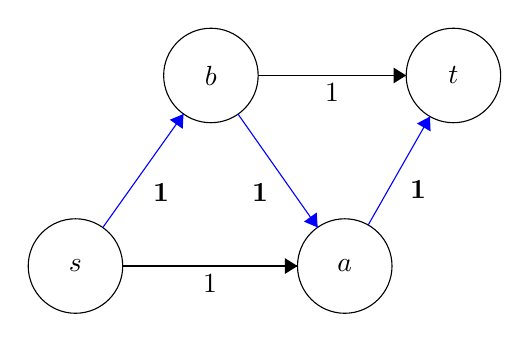
\begin{tikzpicture}[scale=0.2]
  \tikzstyle{every node}+=[inner sep=0pt]
  \draw [black] (5.1,-51.7) circle (3);
  \draw (5.1,-51.7) node {$s$};
  \draw [black] (29.1,-39.6) circle (3);
  \draw (29.1,-39.6) node {$t$};
  \draw [black] (13.7,-39.6) circle (3);
  \draw (13.7,-39.6) node {$b$};
  \draw [black] (22.2,-51.7) circle (3);
  \draw (22.2,-51.7) node {$a$};
  \draw [blue] (6.84,-49.25) -- (11.96,-42.05);
  \fill [blue] (11.96,-42.05) -- (11.09,-42.41) -- (11.91,-42.99);
  \draw (9.99,-47.02) node [right] {\textbf{1}};
  \draw [black] (16.7,-39.6) -- (26.1,-39.6);
  \fill [black] (26.1,-39.6) -- (25.3,-39.1) -- (25.3,-40.1);
  \draw (21.4,-40.1) node [below] {$1$};
  \draw [blue] (15.42,-42.05) -- (20.48,-49.25);
  \fill [blue] (20.48,-49.25) -- (20.42,-48.3) -- (19.61,-48.88);
  \draw (17.36,-47.01) node [left] {\textbf{1}};
  \draw [blue] (23.69,-49.09) -- (27.61,-42.21);
  \fill [blue] (27.61,-42.21) -- (26.78,-42.65) -- (27.65,-43.15);
  \draw (26.31,-46.87) node [right] {\textbf{1}};
  \draw [black] (8.1,-51.7) -- (19.2,-51.7);
  \fill [black] (19.2,-51.7) -- (18.4,-51.2) -- (18.4,-52.2);
  \draw (13.65,-52.2) node [below] {$1$};
  \end{tikzpicture}
  \end{center}
  \vspace{5mm}
  \textbf{Figure C}
  \begin{center}
  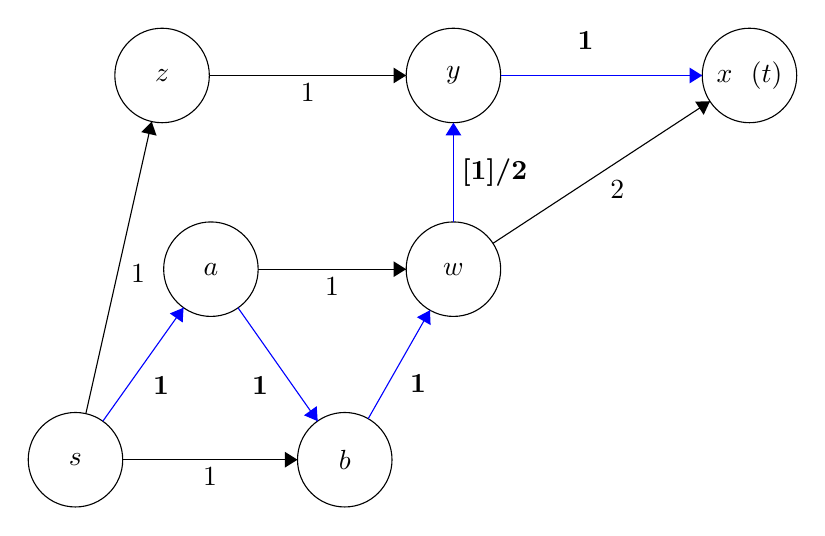
\begin{tikzpicture}[scale=0.2]
  \tikzstyle{every node}+=[inner sep=0pt]
  \draw [black] (5.1,-51.7) circle (3);
  \draw (5.1,-51.7) node {$s$};
  \draw [black] (29.1,-39.6) circle (3);
  \draw (29.1,-39.6) node {$w$};
  \draw [black] (13.7,-39.6) circle (3);
  \draw (13.7,-39.6) node {$a$};
  \draw [black] (22.2,-51.7) circle (3);
  \draw (22.2,-51.7) node {$b$};
  \draw [black] (10.6,-27.3) circle (3);
  \draw (10.6,-27.3) node {$z$};
  \draw [black] (29.1,-27.3) circle (3);
  \draw (29.1,-27.3) node {$y$};
  \draw [black] (47.9,-27.3) circle (3);
  \draw (47.9,-27.3) node {$x~~(t)$};
  \draw [blue] (6.84,-49.25) -- (11.96,-42.05);
  \fill [blue] (11.96,-42.05) -- (11.09,-42.41) -- (11.91,-42.99);
  \draw (9.99,-47.02) node [right] {\textbf{1}};
  \draw [black] (16.7,-39.6) -- (26.1,-39.6);
  \fill [black] (26.1,-39.6) -- (25.3,-39.1) -- (25.3,-40.1);
  \draw (21.4,-40.1) node [below] {$1$};
  \draw [blue] (15.42,-42.05) -- (20.48,-49.25);
  \fill [blue] (20.48,-49.25) -- (20.42,-48.3) -- (19.61,-48.88);
  \draw (17.36,-47.01) node [left] {\textbf{1}};
  \draw [blue] (23.69,-49.09) -- (27.61,-42.21);
  \fill [blue] (27.61,-42.21) -- (26.78,-42.65) -- (27.65,-43.15);
  \draw (26.31,-46.87) node [right] {\textbf{1}};
  \draw [black] (8.1,-51.7) -- (19.2,-51.7);
  \fill [black] (19.2,-51.7) -- (18.4,-51.2) -- (18.4,-52.2);
  \draw (13.65,-52.2) node [below] {$1$};
  \draw [black] (5.76,-48.77) -- (9.94,-30.23);
  \fill [black] (9.94,-30.23) -- (9.28,-30.9) -- (10.25,-31.12);
  \draw (8.6,-39.89) node [right] {$1$};
  \draw [black] (13.6,-27.3) -- (26.1,-27.3);
  \fill [black] (26.1,-27.3) -- (25.3,-26.8) -- (25.3,-27.8);
  \draw (19.85,-27.8) node [below] {$1$};
  \draw [blue] (29.1,-36.6) -- (29.1,-30.3);
  \fill [blue] (29.1,-30.3) -- (28.6,-31.1) -- (29.6,-31.1);
  \draw (29.6,-33.45) node [right] {\textbf{[1]/2}};
  \draw [black] (31.61,-37.96) -- (45.39,-28.94);
  \fill [black] (45.39,-28.94) -- (44.45,-28.96) -- (44.99,-29.8);
  \draw (39.5,-33.95) node [below] {$2$};
  \draw [blue] (32.1,-27.3) -- (44.9,-27.3);
  \fill [blue] (44.9,-27.3) -- (44.1,-26.8) -- (44.1,-27.8);
  \draw (37.5, -24.5) node [below] {\textbf{1}};
  \end{tikzpicture}
  \end{center}
  \vspace{5mm}
  \textbf{Figure D}
  \begin{center}
  \begin{tikzpicture}[scale=0.2]
  \tikzstyle{every node}+=[inner sep=0pt]
  \draw [black] (5.1,-51.7) circle (3);
  \draw (5.1,-51.7) node {$s$};
  \draw [black] (29.1,-39.6) circle (3);
  \draw (29.1,-39.6) node {$c$};
  \draw [black] (13.7,-39.6) circle (3);
  \draw (13.7,-39.6) node {$a$};
  \draw [black] (22.2,-51.7) circle (3);
  \draw (22.2,-51.7) node {$b$};
  \draw [black] (10.6,-27.3) circle (3);
  \draw (10.6,-27.3) node {$d$};
  \draw [black] (29.1,-27.3) circle (3);
  \draw (29.1,-27.3) node {$e$};
  \draw [black] (47.9,-27.3) circle (3);
  \draw (47.9,-27.3) node {$w$};
  \draw [black] (5.1,-12.3) circle (3);
  \draw (5.1,-12.3) node {$z$};
  \draw [black] (47.9,-12.3) circle (3);
  \draw (47.9,-12.3) node {$y$};
  \draw [black] (68.9,-12.3) circle (3);
  \draw (68.9,-12.3) node {$x~~(t)$};
  \draw [blue] (6.84,-49.25) -- (11.96,-42.05);
  \fill [blue] (11.96,-42.05) -- (11.09,-42.41) -- (11.91,-42.99);
  \draw (9.99,-47.02) node [right] {\textbf{1}};
  \draw [black] (16.7,-39.6) -- (26.1,-39.6);
  \fill [black] (26.1,-39.6) -- (25.3,-39.1) -- (25.3,-40.1);
  \draw (21.4,-40.1) node [below] {$1$};
  \draw [blue] (15.42,-42.05) -- (20.48,-49.25);
  \fill [blue] (20.48,-49.25) -- (20.42,-48.3) -- (19.61,-48.88);
  \draw (17.36,-47.01) node [left] {\textbf{1}};
  \draw [blue] (23.69,-49.09) -- (27.61,-42.21);
  \fill [blue] (27.61,-42.21) -- (26.78,-42.65) -- (27.65,-43.15);
  \draw (26.31,-46.87) node [right] {\textbf{1}};
  \draw [black] (8.1,-51.7) -- (19.2,-51.7);
  \fill [black] (19.2,-51.7) -- (18.4,-51.2) -- (18.4,-52.2);
  \draw (13.65,-52.2) node [below] {$1$};
  \draw [black] (5.76,-48.77) -- (9.94,-30.23);
  \fill [black] (9.94,-30.23) -- (9.28,-30.9) -- (10.25,-31.12);
  \draw (8.6,-39.89) node [right] {$1$};
  \draw [black] (13.6,-27.3) -- (26.1,-27.3);
  \fill [black] (26.1,-27.3) -- (25.3,-26.8) -- (25.3,-27.8);
  \draw (19.85,-27.8) node [below] {$1$};
  \draw [blue] (29.1,-36.6) -- (29.1,-30.3);
  \fill [blue] (29.1,-30.3) -- (28.6,-31.1) -- (29.6,-31.1);
  \draw (29.6,-33.45) node [right] {\textbf{[1]/2}};
  \draw [black] (31.61,-37.96) -- (45.39,-28.94);
  \fill [black] (45.39,-28.94) -- (44.45,-28.96) -- (44.99,-29.8);
  \draw (39.5,-33.95) node [below] {$2$};
  \draw [blue] (32.1,-27.3) -- (44.9,-27.3);
  \fill [blue] (44.9,-27.3) -- (44.1,-26.8) -- (44.1,-27.8);
  \draw (38.5,-27.8) node [below] {\textbf{1}};
  \draw [black] (5.1,-48.7) -- (5.1,-15.3);
  \fill [black] (5.1,-15.3) -- (4.6,-16.1) -- (5.6,-16.1);
  \draw (5.6,-32) node [right] {$1$};
  \draw [black] (8.1,-12.3) -- (44.9,-12.3);
  \fill [black] (44.9,-12.3) -- (44.1,-11.8) -- (44.1,-12.8);
  \draw (26.5,-12.8) node [below] {$1$};
  \draw [blue] (47.9,-24.3) -- (47.9,-15.3);
  \fill [blue] (47.9,-15.3) -- (47.4,-16.1) -- (48.4,-16.1);
  \draw (48.4,-19.8) node [right] {\textbf{[1]/3}};
  \draw [black] (50.34,-25.56) -- (66.46,-14.04);
  \fill [black] (66.46,-14.04) -- (65.52,-14.1) -- (66.1,-14.92);
  \draw (59.4,-20.3) node [below] {$3$};
  \draw [blue] (50.9,-12.3) -- (65.9,-12.3);
  \fill [blue] (65.9,-12.3) -- (65.1,-11.8) -- (65.1,-12.8);
  \draw (58.4,-12.8) node [below] {\textbf{1}};
  \end{tikzpicture}
  \end{center}

\end{proof}
\end{problem}
